\documentclass[a4paper]{article}
\usepackage[T1]{fontenc}
\usepackage[utf8]{inputenc}
\usepackage{amsmath}
\usepackage{verbatim}
\usepackage{graphicx}
\usepackage{caption}
\title{\bf A Linearly implicit predictor-corrector scheme for pricing European options}
\date{ April 29, 2018}
\author{Kayode Olumoyin}
\begin{document}
\maketitle

\section{Problem Description}
We considered the the Black-Scholes equation and boundary conditions for a European call with value $C(S,t)$
\begin{equation}\label{ref1}
\frac{\partial C}{\partial t} +  \frac{1}{2}\sigma^2 S^2 \frac{\partial ^2 C}{\partial S^2} + rS \frac{\partial C}{\partial S} -rC = 0
\end{equation}
With 
\[
C(0,t)=0, \qquad C(S,t) \sim S \qquad as  \qquad S \rightarrow \infty \qquad C(S,T)=max(S-E,0)
\]
letting
\[
S=E exp(x), \qquad t=T-\frac{\tau}{\frac{1}{2}\sigma^2}, \qquad C=E exp(x,\tau)
\]
transforms (\ref{ref1}) into a forward in time equation in dimensionless form (Wilmott er al., 1995, Section 5.4) which, using parameter values from Neftci (2000), becomes
\[
\frac{\partial u}{\partial t} = \frac{\partial ^2 u}{\partial x^2} + (c-1) \frac{\partial u}{\partial x} -cu  \qquad t_0 \leq t \leq t_f, \qquad a \leq x \leq b,
\]

where
\[
c=\frac{r}{\frac{1}{2}\sigma^2}, \qquad r=0.065, \qquad \sigma=0.8, \qquad a=ln(\frac{2}{5}) \qquad b=ln(\frac{7}{5}), \qquad t_0=0, \qquad t_f=5
\]
with initial condition
\[
u(x,0)=max(exp(x)-1,0)
\]
and boundary conditions
\[
u(a,t)=0, \qquad u(b,t)=\frac{7-5 exp(-ct)}{5}
\]
We solved numerically with the ETD-Crank-Nicolson method and the linearly implicit method using a space mesh consisting of 40 points and 20 equally spaced time levels. We observe that the Crank-Nicolson method gives oscillatory behavior at $x=0$. The linearly implicit method on the otherhand is oscillation-free everywhere.

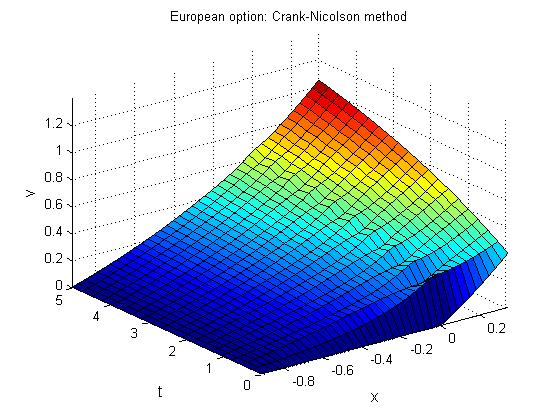
\includegraphics[width=150mm,scale=1.0]{ETDcn.jpg}

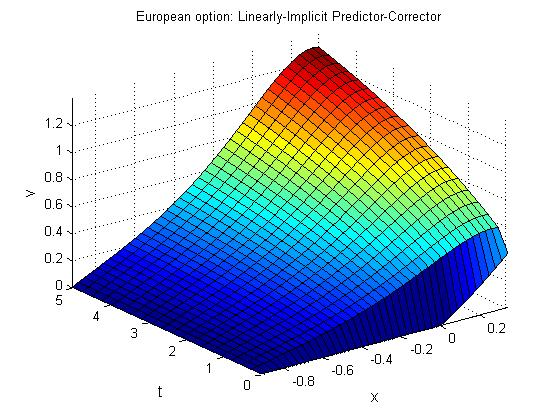
\includegraphics[width=150mm,scale=1.0]{linImpPC.jpg}

\end{document}